This section describes our system by presenting it in different layers, illustrating the layer that captures data on the top, and interacting with the lower-level layer on the bottom, the data processing layer. The Data Capture Layer components both obtain information from the Data Processing Layerr, such as current medication stored in the database, and information inputted by the user from the Data Capture Layer into the Data Processing Layer.  

\begin{figure}[h!]
	\centering
 	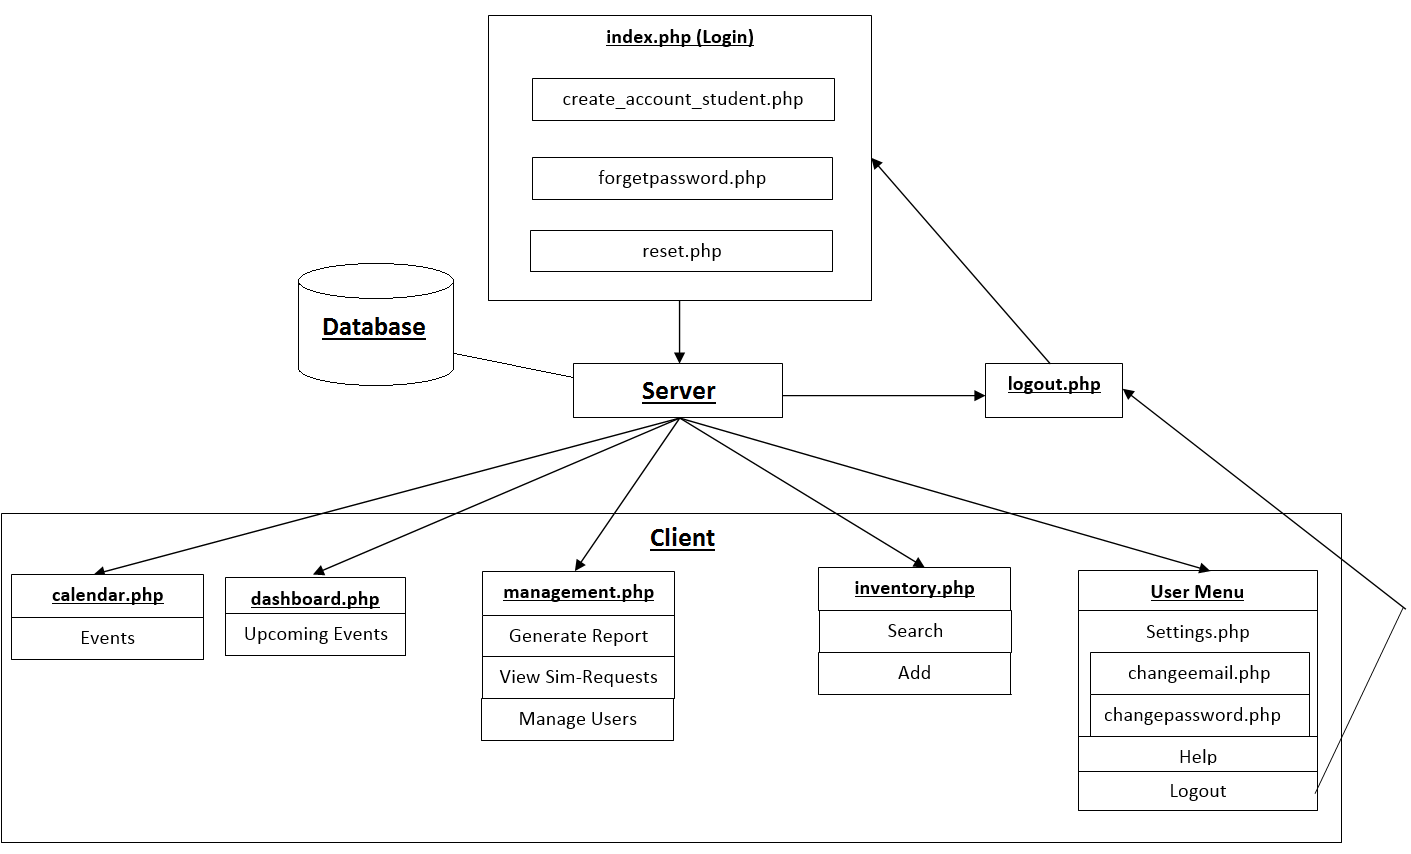
\includegraphics[width=0.3\textwidth]{images/systemoverview}
 \caption{A simple architectural layer diagram}
\end{figure}

\subsection{Client}
This layer takes input from the user and stores it in the database. It also takes data from the database as well as static content for the webpages from the server in order to display the graphical user interface , along with their data, if they have any. Take the inventory page, for example. The client presses on the inventory tab. The server obtains data from the database, such as what the inventory items are, and the static content for the webpages from the server, and these are linked together to have data loaded on the actual graphical user interface to the client. 

\subsection{Server}
This layer contains static information for the webpages, such as the CSS, Bootstrap, HTML, and php code needed to display the web page, and contains the interface that is needed to link the webpages with the data, if they needed any, as described in the client layer.

\subsection{Data}
This layer stores all the information that needs to be used by users of the website, such as the actual inventory items to be stored in the lab. 